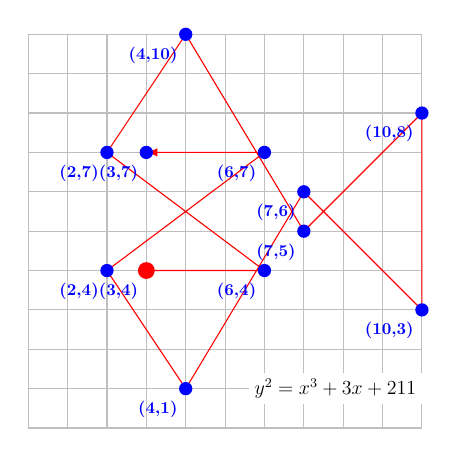
\begin{tikzpicture}[scale=0.5,
every node/.style={scale=0.6}, 
every label/.style={blue},
dot/.style={inner sep=1pt, minimum width=8pt, circle, fill=blue}]

%\draw (0,0) rectangle (10,10);
\draw[step=1cm,gray!50, thin] (0,0) grid (10,10);

%\node (p\i) at (3,4) [inner sep=1pt, minimum width=2pt, circle, fill=blue] {};


\draw [-latex,thin,red] (3,4)
\foreach \p in {(3,4), (6,4), (2,7), (4,10), (7,5), (10,8), (10,3), (7,6), (4,1), (2,4), (6,7), (3,7)}
{ -- \p };


 \foreach \p in {(3,4), (6,4), (2,7), (4,10), (7,5), (10,8), (10,3), (7,6), (4,1), (2,4), (6,7), (3,7)}
 { \node at \p [dot, label=250:{\textbf{\p}}] {}; 
 %\node at \p + (0.2,-0.2) [fill=white] {\p}; 
 }
 
 \node at (3,4) [minimum width=9pt, circle, red, fill=red, draw] {};
\node at (7.8,1) [fill=white] {\large $y^2 = x^3 + 3x + 2 \mod 11 $};

% \foreach \i / \p in { 1 / (3,4), 2 / (6,4), 3 / (2,7), 4 / (4,10), 5 / (7,5), 6 / (10,8), 7 / (10,3),
%     8 / (7,6), 9 / (4,1), 10 / (2,4), 11 / (6,7), 12 / (3,7) }
%  { \node at \p [inner sep=1pt, minimum width=2pt, circle, fill=blue] {}; }

% \node (seed) at (-2,0) [draw=red!70,fill=red!20, inner sep=1pt, minimum width=8pt, circle, label=above:$G(s)$] {};

% \foreach \i in {0,1,...,20}
%     {
%     \node (p\i) at (rand,rand) [inner sep=1pt, minimum width=2pt, circle, fill=blue] {};
%     \draw[-,very thin,red] (seed) parabola (p\i);
%     }

\end{tikzpicture}